\renewcommand{\newCommandChapterTitle}{Introducción}
\chapter{\newCommandChapterTitle}
\markright{\hfill \thechapter. \newCommandChapterTitle}
\label{chap:p3_introduction}


En este capítulo introducimos el tema de este trabajo. Describimos el área
de estudio que rodea nuestra investigación, mostramos la problemática que
nos llevó a realizar este trabajo y presentamos los objetivos que nos
hemos propuesto para el mismo.


\section{Motivación}

Las aplicaciones web han tenido un gran auge en la última década,
convirtiéndose en herramientas de uso masivo y frecuente para una gran
cantidad de usuarios. Pero debido a que las mismas son accesibles a
través de la red, están expuestas a una gran variedad de ataques
\citep{gimenez2015tfg}. % from section 1.1 - motivation
Muchas de las aplicaciones web actualmente no están construidas de acuerdo
a las mejores prácticas de seguridad, posibilitando que  dichas aplicaciones
queden vulnerables a diferentes ataques.
Esto se debe a la falta de consciencia sobre la importancia de la seguridad
y en muchos casos también a una falta de tiempo, ya que se suele priorizar
el desarrollo de funcionalidades por encima de la seguridad. Esta es la
situación de aplicaciones existentes como también lo puede ser para
aplicaciones futuras. Por lo tanto se necesitan soluciones para mitigar
los riesgos presentes
\citep{robertson2009detecting}. % from section 1.1.3 - web culture

En este trabajo nosotros investigamos sobre mecanismos externos
especializados en la detección de ataques, con el fin de mitigar los
riesgos creados por las vulnerabilidades presentes en las aplicaciones
web.
\bigskip

Los sistemas de detección de intrusión (\gls{acr3:ids} - \textit{Intrusion
Detection System}) son programas o dispositivos especializados para
monitorear las actividades en un sistema o en una red en busca de intrusiones
no autorizadas o posibles ataques. Las respuestas frente a intrusiones
pueden ser variadas, como por ejemplo el envío de mensajes de alerta o
incluso medidas concretas de mitigación y contención de los posibles
ataques. En este último caso se puede hablar también más específicamente
de sistemas de prevención de intrusión (\gls{acr3:ips} -
\textit{Intrusion Prevention System})
\citep{scarfone2007guide}. % from section 2 - IDS and IPS principles

Los \gls{acr3:ids} pueden basarse en varias fuentes de datos para sus
análisis, como por ejemplo el tráfico de una red o los registros de
acciones en un sistema operativo
\citep{torranoGimenez2015study}. % from section 2.2.1.2 - classification of location
Como las aplicaciones web utilizan mayormente el protocolo \gls{acr3:http}
(\textit{Hypertext Transfer Protocol}) \citep{fielding1999http} para sus
comunicaciones, se necesita un \gls{acr3:ids} que pueda monitorear el
tráfico \gls{acr3:http}, analizando los mensajes \gls{acr3:http} enviados
y recibidos a través de las conexiones de red.
En este caso se puede hablar más específicamente de cortafuegos para
aplicaciones web (\gls{acr3:waf} - \textit{Web Application Firewall})
\citep{torranoGimenez2015study}. % from section 2.2.3 - wafs

En este trabajo presentamos \gls{acr3:name}, un sistema de detección de
ataques contra aplicaciones web.
Cabe mencionar que debido a que \gls{acr3:waf} es un término más específico
que \gls{acr3:ids}, muchos de los conceptos expuestos en este trabajo
aplican a ambos términos, pero nosotros nos enfocamos en el término
\gls{acr3:waf}.
\bigskip

Los \gls{acr3:waf} pueden utilizar dos métodos distintos para la detección
de intrusiones. Una forma puede ser la búsqueda de patrones de ataques
conocidos, llamado también método basado en firmas de ataques
(\textit{signature-based detection}). Otro método empleado es la búsqueda
de anomalías en los mensajes \gls{acr3:http} con respecto al tráfico
normal, ya que estas desviaciones pueden indicar ataques
(\textit{anomaly-based detection})
\citep{torranoGimenez2015study}. % from section 2.2.1.3 - classification of methodology

Para que un \gls{acr3:waf} pueda utilizar eficazmente el método por
firmas, es necesario que el mismo mantenga una lista actualizada de
las firmas de los ataques conocidos. La lista de firmas de ataques
descubiertos crece constantemente y probablemente nunca deje de crecer.
Durante el análisis de los mensajes, el \gls{acr3:waf} debe tomar en
consideración toda la lista de firmas en busca de ataques, y esta lista
creciente causa que aumente el tiempo de procesamiento y el uso de
recursos para este proceso de detección
\citep{kruegel2003anomaly}. % from section 1 - introduction

El método de detección de anomalías no requiere una lista de firmas,
sino que trabaja en dos fases: entrenamiento y detección. En la fase
de entrenamiento, este tipo de \gls{acr3:waf} construye modelos que
representan a los mensajes \gls{acr3:http} normales. Se basa en la premisa
de que los ataques se diferencian en alguna forma de los mensajes normales.
En adelante usamos el término anomalía para referirnos a los ataques,
para ser consistentes con la literatura relacionada.
Así, durante la fase de detección o monitoreo, este tipo de \gls{acr3:waf}
compara los mensajes nuevos con los modelos construidos anteriormente,
con el fin de detectar desviaciones significativas, es decir, aquellos
mensajes \gls{acr3:http} que son considerados anomalías
\citep{kruegel2003anomaly}. % from section 1 - introduction
La fase de entrenamiento es obligatoria una vez al inicio del uso y
después es necesaria si existen cambios en los mensajes normales, por
ejemplo, luego de la modificación a una o más aplicaciones web protegidas
por el \gls{acr3:waf} en cuestión.

El método por anomalías tiene la ventaja de poder detectar anomalías
debidas a nuevos ataques desde el momento que aparezcan, mientras que
los métodos por firmas dependen de la actualización de su lista de ataques
\citep{kruegel2003anomaly}. % from section 1 - introduction

A pesar de esta importante ventaja, los \gls{acr3:waf}s basados en anomalías
no son tan comunes como aquellos basados en firmas
\citep{sommer2010outside} % from section 1 - introduction
\citep{kruegel2003anomaly}. % from section 1 - introduction
Esto se debe en parte a que suele ser más complicado construir modelos
significativos para diferenciar mensajes normales de anómalos y, como
consecuencia, hay menos posibilidades de detectar eficazmente las anomalías.
De esta manera los métodos por anomalías corren el peligro de caer en
extremos. Por un lado, si se concentran en detectar todas las anomalías
(que son las muestras positivas), pueden marcar equivocadamente mensajes
normales como anómalos (genera más errores de falsos positivos).
Por otro lado, si priorizan no bloquear ningún mensajes normal (que son
las muestras negativas), puede que muchas anomalías no sean detectadas
(genera más errores de falsos negativos)
\citep{torranoGimenez2015study}. % from section 2.2.1.3 - classification of methodology

El \gls{acr3:waf} que presentamos en este trabajo emplea detección de
anomalías en los mensajes \gls{acr3:http}, buscando mejorar algunas de
las propuestas que ya han sido presentadas por otros investigadores,
como por ejemplo \citep{kruegel2003anomaly},
\citep{gimenez2015tfg}, \citep{gimenez2015paper} y
\citep{torranoGimenez2015study}.
\bigskip

Para la detección de anomalías se puede utilizar varias estrategias.
Una opción es emplear herramientas estadísticas, como podemos ver en
los trabajos \citep{kruegel2003anomaly}, \citep{gimenez2015tfg} y
\citep{torranoGimenez2015study}.
Otra opción son herramientas del área de aprendizaje de máquinas
(\gls{acr3:ml} - \textit{Machine Learning}) para tratar de detectar
las anomalías; podemos ver esto en los trabajos \citep{sommer2010outside},
\citep{buczak2016survey}, \citep{parhizkar2015oc}
y \citep{torranoGimenez2015study}.

Las herramientas de \gls{acr3:ml} han sido empleadas con éxito en varias
áreas de la computación, como por ejemplo, en sistemas de recomendación,
clasificación de imágenes, reconocimiento óptico de caracteres, entre
otros \citep{torranoGimenez2015study}. % from section 2.4.2 - ML

Una de las áreas de \gls{acr3:ml} son los problemas de clasificación,
y la detección de anomalías puede ser encarada como un problema de este
tipo. En estos problemas se busca clasificar las muestras en varios grupos
o clases, utilizando una de las herramientas disponibles en \gls{acr3:ml}.
Acá también se observan dos fases, una de entrenamiento y otra de detección
o clasificación.
En este contexto se habla de aprendizaje supervisado si se especifican
todas las clases posibles de antemano, usando solamente muestras para el
entrenamiento de las que se conocen sus clases; muestras nuevas serán
asignadas a la clase a la que más se parezcan. En cambio, se habla de
aprendizaje no supervisado cuando no se provee muestras con clases conocidas
de antemano y la herramienta debe tratar de encontrar las clases presentes
\citep{torranoGimenez2015study}. % from section 2.4.2 - ML
También se puede dar el caso de que se conozca las clases de solamente
algunas de las muestras, o que se tenga únicamente muestras de una clase
conocida pero no se tenga muestras de las demás clases; en estos casos
se puede hablar de aprendizaje semi-supervisado
\citep{aggarwal2013outlier}. % from section 7.4 - Semi-Supervision

Aplicado a un \gls{acr3:waf}, se puede usar clasificación supervisada,
definiendo una clase para los mensajes normales y otra clase (o también
varias otras clases) para los mensajes anómalos.
Un primer desafío con este abordaje es que se necesita volver a entrenar
el clasificador cuando aparece un nuevo tipo de anomalía. Si no se vuelve
a entrenarlo con muestras que contengan los nuevos tipos de anomalías, es
posible que una anomalía sea clasificada equivocadamente como un mensaje
normal en el caso de una anomalía nueva que no se ajusta suficientemente
a las clases de anomalías con las cuales el clasificador fue entrenado
anteriormente.
Un segundo desafío con este abordaje es la necesidad de obtener muestras
de todos los tipos de anomalías conocidas para poder realizar un
entrenamiento completo.

Estos dos desafíos se trata de superar con la estrategia conocida bajo
el nombre de clasificación de una sola clase (\gls{acr3:occ} -
\textit{One-Class Classification})
\citep{khan2009survey}. % from section 1 - introduction
Se busca definir una sola clase, la clase conocida, y clasificar las
muestras de acuerdo a si pertenecen o no a dicha clase. La fase de
entrenamiento utiliza solamente muestras de la clase conocida, con la
finalidad de que en la fase de detección las muestras que no se ajusten
a la clase conocida sean clasificadas como no perteneciente a la misma.
Esto provee robustez al clasificador frente a la aparición de novedosas
muestras que no pertenecen a la clase conocida.
Esta estrategia ha sido utilizada con éxito en varias áreas, como detección
de spam, reconocimiento de rostros, detección de fallas en maquinarias,
entre otros \citep{khan2014one}. % from section 4.3.2 - application domains
Aplicado a un \gls{acr3:waf}, la clase conocida esta conformada solamente
por los mensajes normales y todos los tipos de anomalías que representan
los distintos tipos de ataques no pertenecerán a dicha clase. Para ser
consistentes con la terminología del área de seguridad, las anomalías o
ataques son las muestras positivas, que no pertenecerán a la clase conocida
de los mensajes normales (que son las muestras negativas).

Este trabajo presenta \gls{acr3:name}, que emplea \gls{acr3:occ} con
herramientas de \gls{acr3:ml} para detectar mensajes anómalos. Con este
abordaje solamente se necesita realizar una vez el entrenamiento con
mensajes normales y, mientras no cambien las aplicaciones protegidas,
no debería ser necesario volver a entrenarlo, aún con la aparición de
nuevos ataques.
\bigskip

Los algoritmos o herramientas utilizados en \gls{acr3:ml} son muy diversos,
como por ejemplo
árboles de decisiones \citep{torranoGimenez2015study}, % from section 2.4.2 - ML
redes neuronales \citep{corchado2011neural},
algoritmos genéticos \citep{abadeh2011design},
entre otros \citep{torranoGimenez2015study}. % from section 2.4.2 - ML
Una de estas herramientas, que ha sido utilizada con mucho éxito en las
tareas de clasificación, es la máquina de vectores de soporte
(\gls{acr3:svm} - \textit{Support Vector Machine}). Una versión modificada
del \gls{acr3:svm} ha sido propuesta como una de varias alternativas
para afrontar tareas de \gls{acr3:occ} \citep{scholkopf2001estimating}.
Varios investigadores ya han empleado exitosamente este clasificador
\gls{acr3:ocsvm} en problemas de diversas áreas, como por ejemplo en
clasificación de textos y rostros, detección de spam, detección de fallas
en máquinas, entre otros
\citep{khan2014one}. % from section 4.3.2 - application domains

El detector \gls{acr3:name} presentado en este trabajo utiliza clasificadores
\gls{acr3:ocsvm} para detectar mensajes \gls{acr3:http} anómalos.
\bigskip

Para que un \gls{acr3:waf} basado en detección de anomalías pueda diferenciar
los mensajes \gls{acr3:http} normales de los anómalos, es necesario que
existan características de dichos mensajes que posibiliten esa diferenciación.
Ejemplos de esos rasgos pueden ser la longitud de la petición, la presencia
de ciertos caracteres con significado especial, la distribución de la
frecuencia de los caracteres, entre otros
\citep{kruegel2003anomaly}. % from section 4 - detection models
Además se debe expresar esas características en un formato procesable
para las herramientas de detección. La mayoría de las herramientas de
\gls{acr3:ml}, incluyendo el clasificador \gls{acr3:ocsvm}, no pueden
trabajar con los datos crudos y necesitan un paso de preprocesamiento
de datos.
Asumiendo la existencia de esas características distintivas, el éxito
del \gls{acr3:waf} depende de encontrar dichas características y de
representarlas en un formato procesable para el mecanismo de detección
\citep{torranoGimenez2015study}. % from section 2.3.1 - feature extraction
En esta parte, el conocimiento experto sobre los mensajes \gls{acr3:http}
ayuda a seleccionar las características más útiles para el proceso de
detección. Podemos ver un ejemplo de esta selección de características
en los trabajos \citep{kruegel2003anomaly} y \citep{kruegel2005multi},
donde se utiliza conocimiento sobre la estructura de mensajes para obtener
características más específicas y así mejorar los resultados de la
detección.

Para el clasificador \gls{acr3:ocsvm}, esas características de los mensajes
\gls{acr3:http} se deben representar con vectores numéricos, llamados
también vectores de características o \textit{features}. Por ejemplo,
el primer valor del vector puede indicar la cantidad de caracteres del
mensaje \gls{acr3:http}, el segundo la cantidad de dígitos presentes y
el tercero puede representar la longitud de todo el mensaje.
De esta forma, la eficacia de detección de anomalías del clasificador
\gls{acr3:ocsvm} depende en gran parte de nuestros procesos de extracción
de características, es decir, de los procesos de preprocesamiento que
extraen las características distintivas de los mensajes y las representan
como vectores numéricos
\citep{torranoGimenez2015study}. % from section 2.3.1 - feature extraction

En este trabajo presentamos \gls{acr3:name}, que utiliza conocimiento
experto sobre los mensajes \gls{acr3:http} para extraer características
útiles para la detección de anomalías.
Debido a que trabajamos con clasificadores \gls{acr3:ocsvm}, en este
trabajo utilizamos el término \textit{feature} para referirnos a las
características extraídas de los mensajes, para ser consistentes con
la terminología del área de \gls{acr3:ml}.


\section{Justificación}

Resumiendo lo expuesto anteriormente, en este trabajo combinamos tres
áreas de estudio para proponer una solución a la problemática descrita.
Dichas áreas se pueden observar también en la \autoref{fig:intro:areas_de_estudio}.

\begin{figure}[ht]
    \centering
    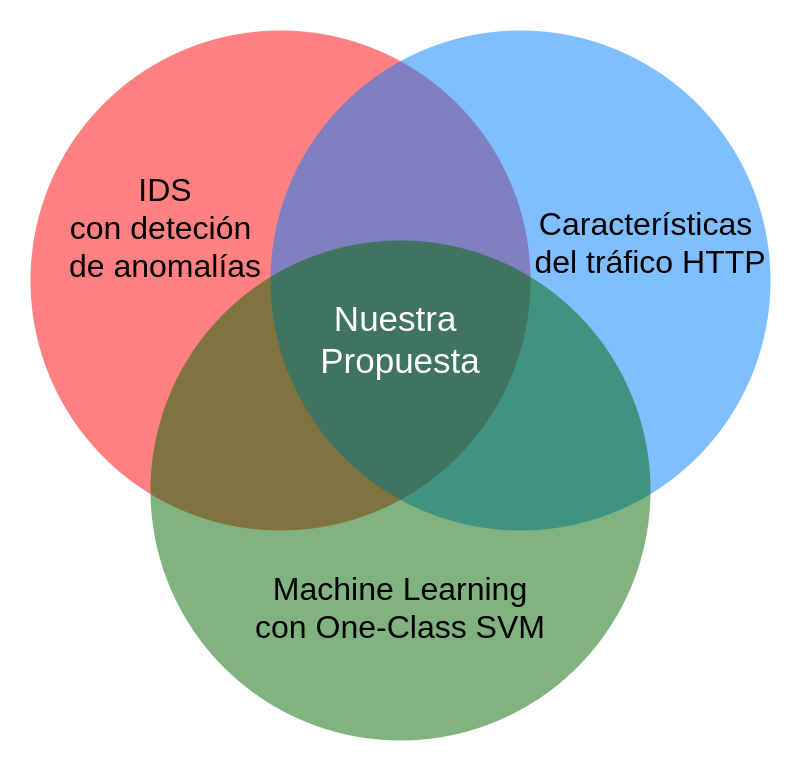
\includegraphics[width=0.5\linewidth]{images/venn-areas-de-estudio.png}

    \caption{Diagrama de las áreas de estudio de la investigación.}
    \label{fig:intro:areas_de_estudio}
\end{figure}

\begin{itemize}
    \item
    \gls{acr3:ids} con detección de anomalías:
    \gls{acr3:name} busca detectar posibles ataques al reconocerlos como
    mensajes anómalos. Utilizamos el método de detección de anomalías
    debido a sus ventajas que fueron mencionadas en la sección anterior.

    \item
    Características de los mensajes \gls{acr3:http}:
    \gls{acr3:name} utiliza conocimiento experto sobre la estructura de
    los mensajes \gls{acr3:http}, que puede ayudar para diferenciar los
    mensajes normales de las anomalías o ataques, como se puede observar
    en los trabajos  \citep{kruegel2003anomaly} y \citep{kruegel2005multi}.

    \item
    \gls{acr3:ml} con \gls{acr3:ocsvm}:
    la detección de mensajes anómalos se puede abordar como un problema
    de \gls{acr3:occ}, y para ese tipo de problemas el clasificador en
    cuestión ha sido empleado exitosamente por otros investigadores,
    obteniendo buenos resultados en la clasificación
    \citep{khan2014one}. % from section 4.3.2 - application domains
\end{itemize}

En los trabajos de Kruegel y Vigna se combina las dos primeras áreas
descritas anteriormente, \gls{acr3:ids} y características de los mensajes
\gls{acr3:http}. Sus aportes ya fueron utilizados y extendidos en varios
trabajos en años subsecuentes, pero nosotros no hemos encontrado una
investigación que combine dichos aportes con el ya mencionado clasificador
\gls{acr3:ocsvm}.

En nuestra opinión, un \gls{acr3:waf} que combina los aportes de Kruegel
y Vigna con este clasificador puede ser de gran utilidad para la detección
de posibles ataques y de esta forma brindar una herramienta para mayor
protección de las aplicaciones web.


\section{Objetivos}

\subsection{Objetivo general}

Detectar mensajes \gls{acr3:http} anómalos entre las aplicaciones web
y sus usuarios con el fin de mitigar los riesgos de ataques contra dichas
aplicaciones, utilizando un \gls{acr3:waf} basado en clasificadores
\gls{acr3:ocsvm}.


\subsection{Objetivos específicos}

\begin{enumerate}
    \item
    Diseñar procesos de extracción de características (\textit{features})
    específicamente para mensajes \gls{acr3:http}, basado en aportes de
    otros investigadores de la literatura.

    \item
    Implementar un \gls{acr3:waf} basado en anomalías, utilizando los
    procesos de extracción de \textit{features} diseñados junto con
    clasificadores \gls{acr3:ocsvm}.

    \item
    Evaluar la eficacia del \gls{acr3:waf} implementado en cuanto a la
    detección de mensajes \gls{acr3:http} anómalos.

    \item
    Analizar la viabilidad de utilizar el \gls{acr3:waf} implementado
    para detección de ataques en tiempo real.
\end{enumerate}


\section{Organización del trabajo}

Este trabajo está organizado de la siguiente manera:
en el \autoref{chap:p3_concepts_features} entramos en más detalles sobre
cómo utilizamos las características de los mensajes \gls{acr3:http} en
nuestros procesos de extracción de \textit{features}.
Luego, en el \autoref{chap:p3_concepts_ocsvm} describimos con más detalles
el clasificador \gls{acr3:ocsvm}, mostrando de qué manera lo empleamos
para la detección de mensajes anómalos.
El \autoref{chap:p3_new_waf} contiene la presentación del \gls{acr3:waf}
que construimos en el marco de este trabajo, describiendo varios detalles
de la implementación y mostrando de qué manera utilizamos los componentes
descritos en los capítulos \ref{chap:p3_concepts_features} y
\ref{chap:p3_concepts_ocsvm}.
Después de eso, en el \autoref{chap:p3_results}, describimos las pruebas
realizadas con nuestra implementación y exponemos los resultados que hemos
obtenido en cada una de ellas.
Finalizamos el presente trabajo con nuestras conclusiones en el
\autoref{chap:p3_conclusions}, agregando también algunas ideas que pueden
ser el punto de partida para trabajos futuros.
